% !TEX root = main.tex

\section{はじめに}
ムーアの法則の終焉により,CPUのコア単体性能は限界に達しつつある.
一方で,IT技術の発展に伴い管理すべきデータは爆発的に増えつつある.
この状況に対処するため,現在のコンピュータ技術は複数のコアを用いて処理を行うマルチスレッド処理が主流である.
データベース分野においても例外ではなく,近年メニーコアなどを前提としたインメモリデータベースの研究が進んでいる.
データベースの構成要素の1つである索引技術も同様に,メニーコア・大容量メモリに適合させる必要がある.

代表的な索引構造である\Bptree{}~\cite{book:dbsystem}では,ロックを用いた同時実行制御が行われている.
しかし,マルチスレッド処理においてロックによる同時実行制御は多数の待ちスレッドが発生するため,スケーラビリティが悪化する.
そこで,\Bptree{}をロックフリー化させた索引としてBw木~\cite{book:Bwtree}やBz木~\cite{book:Bztree},著者らの研究室で開発しているロックフリーB+木(\Bctree{})が提案されている.

また,インターネットの普及に伴いURLの管理やECサイトにおける文字列検索など,特定のキーに対し効率的に処理する索引構造が求められている.
Mass木~\cite{book:Masstree}は,文字列型や整数型などのバイナリ比較可能なキーに特化した索引構造の1~つである.
\Bptree{}を階層的に作成することにより,キャッシュ効率を改善している.

本研究の\Bcforest{}では,著者らの研究室で開発しているロックフリーB+木(\Bctree{})に対し,Mass木のと同様の拡張および性能改善を行う.
特に,本論文ではその構造および操作について述べる.

本稿の構成は以下の通りである.
\Sec{\ref{sec:relatedwork}}では,関連研究としてロックフリー索引やバイナリ比較可能なキーに対し最適化した索引について概説する.
次に,\Sec{\ref{sec:bc_forest_structure}}で\Bcforest{}の構造について説明し,\Sec{\ref{sec:node_operation}}および\Sec{\ref{sec:smo}}で\Bcforest{}の操作について述べる.
最後に,\Sec{\ref{sec:conclusion}}で本稿のまとめと今後の方針を述べる.

Mass木は\Bptree{}にトライ木構造を適応させることで,キャッシュ効率を改善させた.
\Bcforest{}では\Bctree{}に対し,同様の改善を図る.

Mass木の観点では\Bptree{}から\Bctree{}になることにより,ロックフリーによる書き込み性能の改善を図る.
また\Bctree{}の観点では,整数型や文字列型などのバイナリ比較可能なキーに対し,キャッシュ効率の改善を図る.

\section{関連研究}
\label{sec:relatedwork}
関連の深い索引構造として,同時実行制御においてロックを取得しない\Bctree{},および\Bptree{}にトライ木の構造を組み合わせたMass木について紹介する.

\subsection{\Bctree{}}
\Bctree{}はマッピングテーブル,ノード内バッファという構造上の特徴とCAS命令を用いたロックフリー索引である.
\Bctree{}の概形を\Fig{\ref{fig:bc_tree-structure}}に示す.

\begin{figure}[t]
    \centering
    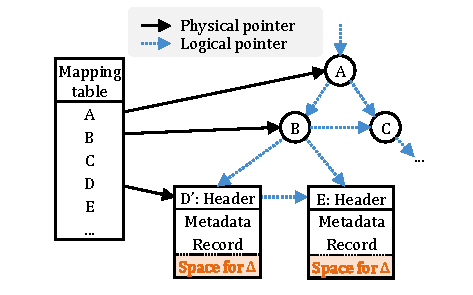
\includegraphics{./figures/Bc-structure.pdf}
    \caption{\Bctree{}の概形}
    \label{fig:bc_tree-structure}
\end{figure}

\subsubsection{データ構造の概観}
\Bptree{}と同様に,\Bctree{}は索引層およびデータ層によって構成される.
索引層のノード(中間ノード)は分割キーと子ノードへのポインタの組を格納し,木の下方への検索を補助する.
構造は\Blinktree{}に則っており,各ノードが同じ階層の右兄弟への参照リンクを持つ.
ノード間の繋がりはマッピングテーブルにより仮想化する.
各ノードは自身の子ノードや兄弟ノードへのポインタを直接持つ代わりにマッピングテーブル上のID(logical page ID, LPID)を持つ.
各ノードへの参照はマッピングテーブルを用いた間接参照を採用し,マッピングテーブル内の物理ポインタを差し替えることでそのノードへの参照を一括で変更する.

各ノードの領域は不変領域と可変領域(ノード内バッファ)に分けられる.
不変領域はノードヘッダおよびソート済みのレコードを格納する.
ヘッダは不変領域の情報を管理し,構造変更時のみその値が変更される.
可変領域はステータスワードの格納と差分レコードを挿入するための書き込みバッファの役割を果たす.
ステータスワードは可変領域の情報を管理し,ノードの現在の状態や残容量などを管理する.

\subsubsection{レコード操作の概観}
ステータスワードをCAS命令で更新することによって,ロックフリーな書き込みを実現している.
各ノードへ構造変更操作を行う際は,構造変更後のノードから構造変更前のノードへ物理リンクを張り,古いノードへの参照を可能にする.

\subsection{Mass木}
Mass木は\Bptree{}を基本単位とした階層構造やレコードメタデータの削除により,キャッシュ効率を改善した索引構造である.
Mass木の概形を\Fig{\ref{fig:masstree}}に示す.

\begin{figure}[t]
    \centering
    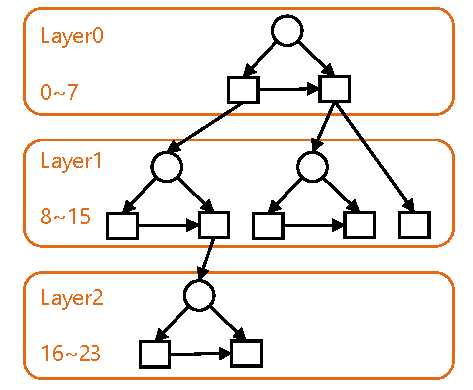
\includegraphics{./figures/masstree.pdf}
    \caption{Mass木の概形}
    \label{fig:masstree}
\end{figure}

Mass木は複数の\Bptree{}とlayer構造から構成される.
Layer~0はキーの先頭0~7~byteで構成される\Bptree{}である.
先頭8~byteで一意性が確保できる場合には,Layer~0で完結する.
先頭8~byteで一意性が確保出来ない場合,Layer~1(キーの8~15~byteで構成される\Bptree{})を作成し,Layer~0からLayer~1への物理リンクを張る.
同様にして,複数の\Bptree{}やLayerを作成し,トライ木に似た構造を持つのがMass木の特徴である.
Mass木は整数型や文字列型など,分割が可能なキーに限定することで上記に示す階層化(共通部分の集約)を可能にしている.

また,Mass木は固定長キーおよび固定長ペイロードに特化したノードレイアウトを利用している.
\Bctree{}のような可変長キーおよび可変長ペイロードに対応する索引構造では,各レコードに対応する固定長レコードメタデータを利用することでノード内のレコードの配置等を管理している.
Mass木では,8~byte分割によりキーが8~byteで固定される.
更に,ペイロードに関してもポインタの活用やインラインを固定長に限定することで,メタデータの利用を回避している.

以上のトライ木構造の利用やレコードメタデータの削除により,Mass木はキャッシュ効率を改善している.

\section{\Bcforest{}の構造}
\label{sec:bc_forest_structure}

\Bcforest{}はBc木をバイナリ比較可能なキーに最適化した索引構造である.
Mass木のように8~byte単位でキーを分割,階層分けし,各階層でのレコード管理にはBc木を利用する.
つまり,各Bc木の中間ノードでは固定長の部分キーおよび子ノードへのポインタのみを管理することとなり,レコードメタデータの除外によるキャッシュ効率の改善が可能となる.
一方で,葉ノードではposting listを用いて共通する部分キーを持つレコードを管理し,少数のレコードのみからなる下層の生成を抑制する.

\subsection{中間ノードにおけるレコードメタデータの除外}
\Bcforest{}では中間ノードはキーを8~byteで分割しているため,固定長キーとして扱うことが出来る.
また,ペイロードは子ノードへのポインタであるため固定長である.
この特性を利用し,\Bcforest{}内の\Bctree{}における中間ノード内のレコードメタデータの除外を行う.
これにより,索引層における探索性能の改善及びキャッシュ効率を改善を図る.

\subsection{葉ノードにおけるposting listの導入}

\begin{figure*}[t]
    \centering
    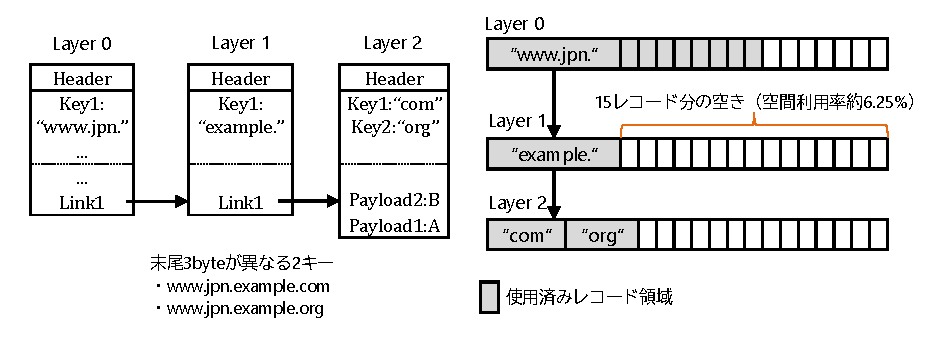
\includegraphics{./figures/memory.pdf}
    \caption{Mass木の空間利用率}
    \label{fig:memory}
\end{figure*}

Mass木においては,空間利用効率が問題となる.
\Fig{\ref{fig:memory}}は末尾3~byteが異なる19~byteの2~キーを格納したMass木の索引構造である.
先頭8~byteが共通するため,layer~1を作成する.
同様に8~16~byte目が共通するため,layer~2を作成する.
Mass木では本来,1~つのノードに最大16~個のレコードを格納することが出来る.
しかしlayer~1では,1~つのレコードしか格納されていない状態でlayer~2を作成している.
layer~1にのみ注目すると,空間利用率は約6.25~\%しかない.

\begin{figure}[t]
    \centering
    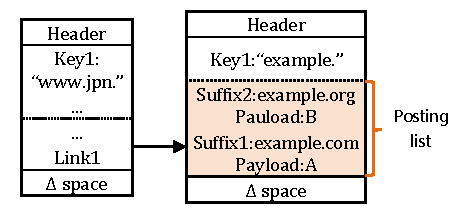
\includegraphics{./figures/posting_list.pdf}
    \caption{posting listの導入}
    \label{fig:posting_list}
\end{figure}

\Bcforest{}では空間利用率の改善として,posting listを導入する.
posting listでは,1~つのキーに対して複数のペイロードを対応付けることが出来る.
\Fig{\ref{fig:posting_list}}はposting listを導入した際の索引構造を示したものである.
layer~1においてposting list作成することで,layer~2の無駄な階層化と空間利用率の悪化を防ぐ.


\section{\Bcforest{}のノード操作}
\label{sec:node_operation}

\subsection{書き込み}

\subsection{読み取り}

\section{\Bcforest{}の構造変更操作}
\label{sec:smo}

\subsection{統合}
\subsection{分割}
\subsection{新層作成}

\section{おわりに}
\label{sec:conclusion}
本稿では\Bctree{}にMass木と同様のトライ木構造を適応させた\Bcforest{}について提案し,その構造および操作を紹介した.
今後は提案した索引構造を実装するとともに,Mass木や近年提案されているBw木やBz木といったロックフリー索引との性能を比較検証する.